\documentclass[11pt]{article}
\usepackage{caption}
\usepackage{anysize}
\usepackage{fancyhdr}
\usepackage{graphicx}
\usepackage{subcaption}
\usepackage{color}
\usepackage{balance}
\usepackage{lipsum}
\usepackage{multirow}
\usepackage{multicol}
\usepackage{booktabs}

% REQUIRED PACKAGES FOR TIKZ DRAWINGS %
\usepackage{tikz}
\usetikzlibrary{positioning}
\usetikzlibrary{spy}
\usetikzlibrary{decorations.fractals}

\marginsize{.75in}{.75in}{.75in}{1in}
\pagestyle{fancy}
\rhead{\today}
\lhead{
\includegraphics[height=2.0cm]{../logo.jpg}}
\rfoot{\thepage}
\cfoot{}
\renewcommand{\headrulewidth}{0pt} %removes line from fancy header
\renewcommand{\thispagestyle}[1]{} %placers header and footer on first page 
\renewcommand{\abstractname}{Summary}
\setlength{\columnsep}{25pt}
\date{}
\title{Laboratory Gasification Diagrams}

\begin{document}
\maketitle

%% %%%%%%%%%  %%
%% Furnace and Tube %%
%% %%%%%%%%%  %%

\begin{center}
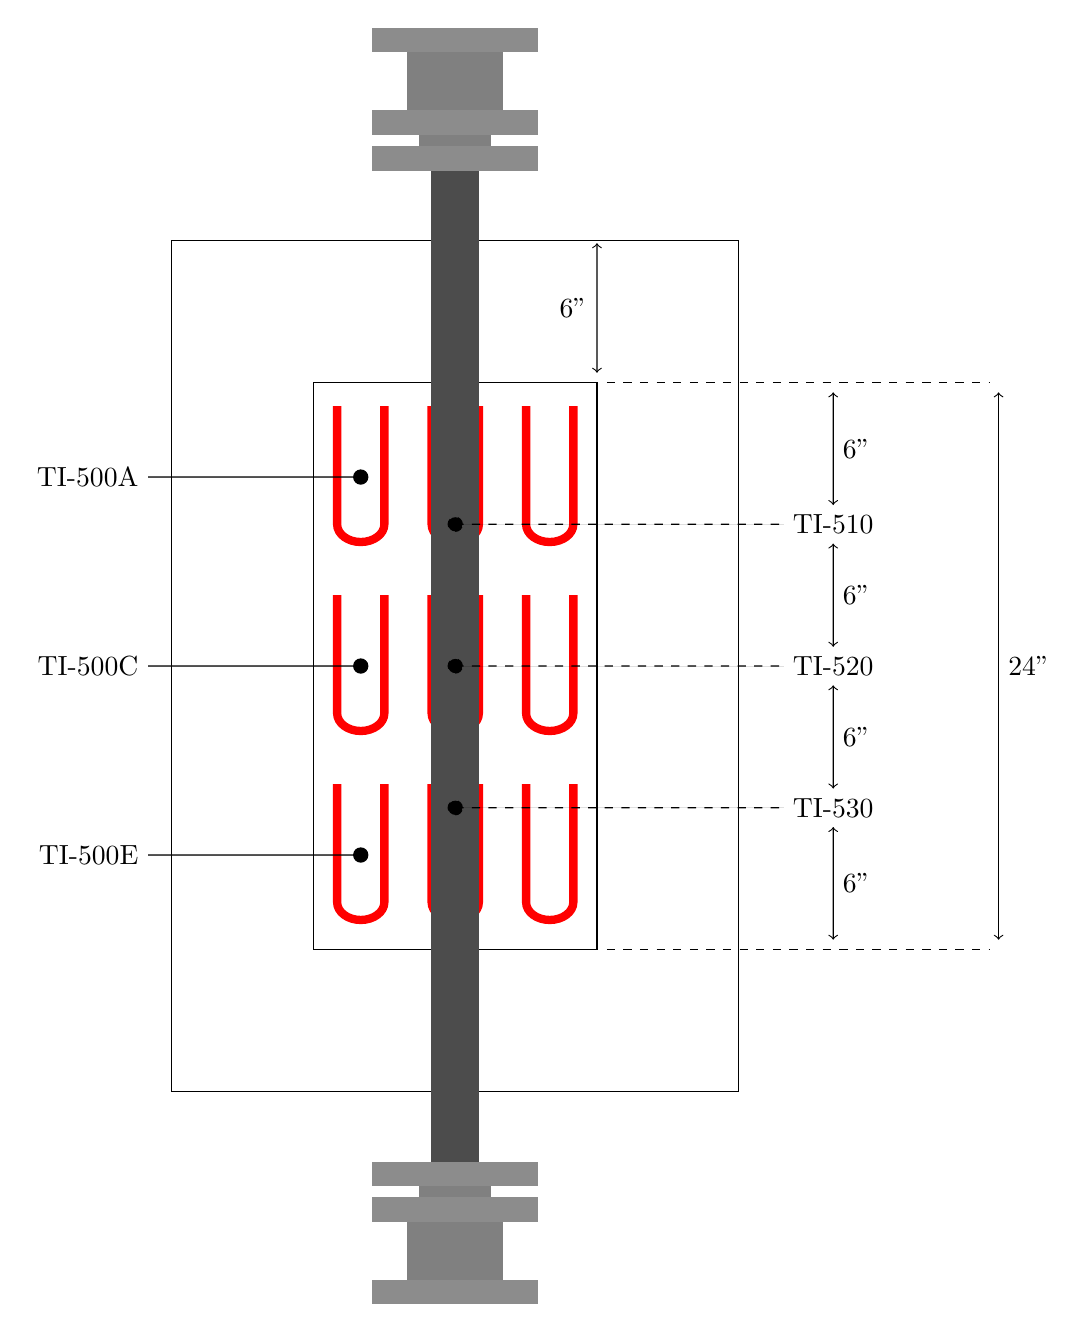
\begin{tikzpicture}[scale=0.3]
	\node (toprighthot) at (6,12) {};
	\node (bottomlefthot) at (-6,-12) {};
	\node (bottomrighthot) at (6,-12) {};
	\node (toplefthot) at (-6,12) {};
	\node (toprightbox) at (12,18) {};
	\node (topleftbox) at (-12,18) {};
	\node (bottomleftbox) at (-12,18) {};
	\node (bottomrightbox) at (12,-18) {};
	% Furnace Box %
	\draw (-12,-18) rectangle  (12,18);
	% Hot Zone %
	\filldraw [fill=red, fill opacity=0.0] (bottomlefthot) rectangle (toprighthot);
	% Elements %
	\foreach \y in {11, 3, -5}
		\foreach \x in {-5, -1, 3}
			{\draw [red,line width=3] (\x,\y) -- ++(0,-5) arc (180:360:1 and 0.75) -- ++(0,5);}
	% Tube %
	\filldraw [black!70!white] (-1,-27) rectangle (1,27);
	% Top Bucket %
	\filldraw [gray] (-1.5,21) rectangle (1.5,23.5);
	\filldraw [gray] (-2,23.5) rectangle (2,27);
	\filldraw [gray!90!white] (-3.5,21) rectangle (3.5,22);
	\filldraw [gray!90!white] (-3.5,22.5) rectangle (3.5,23.5);
	\filldraw [gray!90!white] (-3.5,26) rectangle (3.5,27);
	% Bottom Bucket %
	\filldraw [gray] (-1.5,-21) rectangle (1.5,-23.5);
	\filldraw [gray] (-2,-23.5) rectangle (2,-27);
	\filldraw [gray!90!white] (-3.5,-21) rectangle (3.5,-22);
	\filldraw [gray!90!white] (-3.5,-22.5) rectangle (3.5,-23.5);
	\filldraw [gray!90!white] (-3.5,-26) rectangle (3.5,-27);
	% Skin Thermocouples %
	\filldraw [black] (0,6) circle (0.3) [dashed] -- (16,6) node (ti510) [fill=white] {TI-510};
	\filldraw [black] (0,0) circle (0.3) [dashed] -- (16,0) node (ti520) [fill=white] {TI-520};
	\filldraw [black] (0,-6) circle (0.3) [dashed] -- (16,-6) node (ti530) [fill=white] {TI-530};
	\node (top510) at (16,12) {};
	\node (topright510) at (23,12) {};
	\node (bottom530) at (16,-12) {};
	\node (bottomright530) at (23,-12) {};
	\draw [<->] (top510) to node [auto] {6"} (ti510);
	\draw [<->] (ti510) to node [auto] {6"} (ti520);
	\draw [<->] (ti520) to node [auto] {6"} (ti530);
	\draw [<->] (ti530) to node [auto] {6"} (bottom530);
	\draw [<->] (topright510) to node [auto] {24"} (bottomright530);
	\draw [dashed] (toprighthot) -- (topright510);
	\draw [dashed] (bottomrighthot) -- (bottomright530);
	\draw [<->] (toprighthot) to node [auto] {6"} ++(0,5.9);
	% Element Thermocouples %
	\filldraw [black] (-4,8) circle (0.3) -- (-13,8) node (ti510) [anchor=east] {TI-500A};
	\filldraw [black] (-4,0) circle (0.3) -- (-13,0) node (ti520) [anchor=east] {TI-500C};
	\filldraw [black] (-4,-8) circle (0.3) -- (-13,-8) node (ti530) [anchor=east] {TI-500E};

\end{tikzpicture}
\end{center}

%% %%% %%
%% Lance %%
%% %%% %%	
	
\begin{center}
\begin{tikzpicture}[scale=0.3]

\end{tikzpicture}
\end{center}


%% %%%%%%%  %%
%% Flow Diagram %%
%% %%%%%%%  %%

\begin{center}
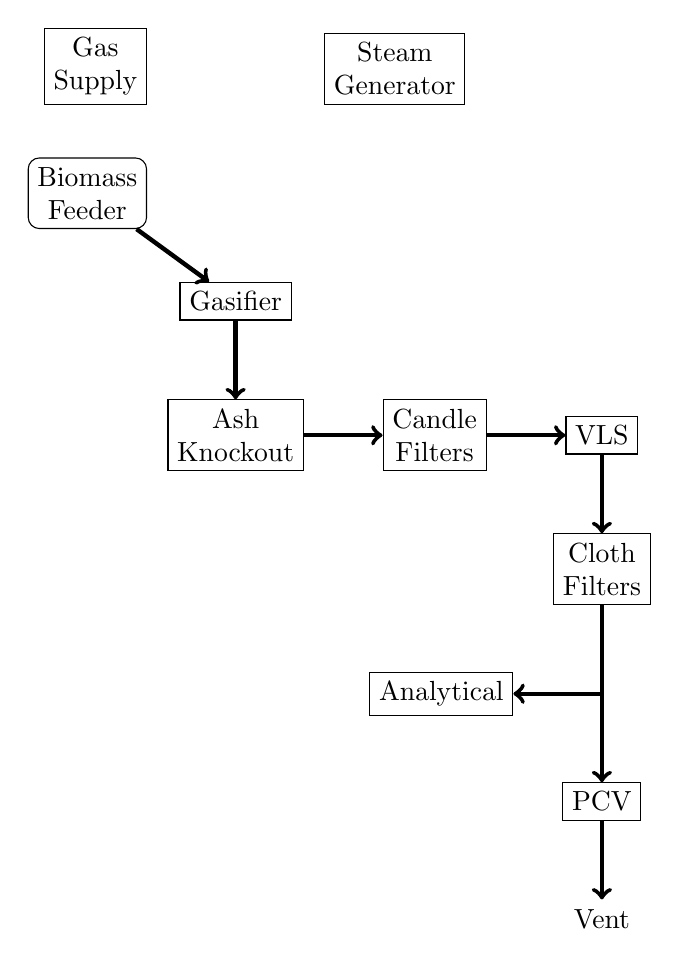
\begin{tikzpicture}[scale=1,
	box/.style={rectangle,draw,align=center}
	]
	\node [box] (gasifier)	{Gasifier};
	\node (lance)			[above=of gasifier]	{};
	\node [box] (ako)		[below=of gasifier]	{Ash \\ Knockout};
	\node [box] (filters)		[right=of ako]		{Candle \\Filters};
	\node [box] (vls)		[right=of filters]	{VLS};
	\node [box] (fabfilters)	[below=of vls]		{Cloth \\ Filters};
	\node (tee)			[below=of fabfilters]	{};
	\node [box] (pcv)		[below=of tee]		{PCV};
	\node [box,rounded corners] (feeder)		[left=of lance]	{Biomass \\Feeder};
	\node [box] (analytical)	[left=of tee]		{Analytical};
	\node (vent)			[below=of pcv]		{Vent};
	
	\node [box] (gas)		[above left=of lance]	{Gas \\ Supply};
	\node [box] (steam)		[above right=of lance]	{Steam \\ Generator};
	
	\draw [->] (feeder) [ultra thick] 				to (gasifier);
	\draw [->] (gasifier) [ultra thick] 			to (ako);
	\draw [->] (ako) [ultra thick] 				to (filters);
	\draw [->] (filters) [ultra thick] 				to (vls);
	\draw [->] (vls) [ultra thick] 				to (fabfilters);
	\draw [->] (fabfilters) [ultra thick] 			to (pcv);
	\draw [->] (tee.center) [ultra thick] 	to (analytical);
	\draw [->] (pcv) [ultra thick]				to (vent) ;

\end{tikzpicture}
\end{center}


%% %%%%%%%%  %%
%% Biomass Feeder %%
%% %%%%%%%%  %%

\begin{center}
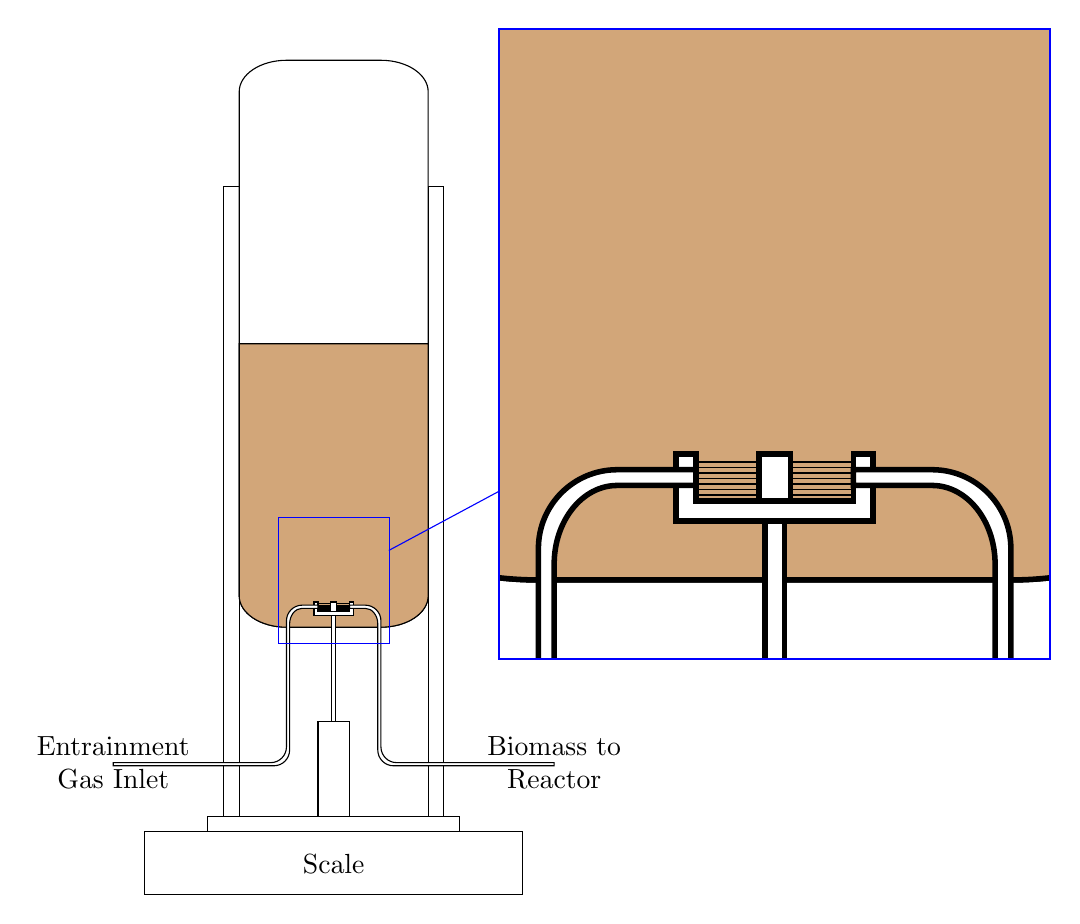
\begin{tikzpicture}[scale=0.2,
	spy using outlines={rectangle, magnification=5, width=7cm, height=8cm, connect spies}]

	% Vessel %
	\draw (-6,-	16) -- (-6,16) arc (180:90:3 and 2) -- (3,18) arc (90:0:3 and 2) -- (6,16) -- (6,-16) arc (0:-90:3 and 2) -- (-3,-18) arc  (-90:-180:3 and 2);
	\draw [fill=brown!70!white] (-6,-16) -- (-6,0) -- (6,0) -- (6,-16) arc (0:-90:3 and 2) -- (-3,-18) arc  (-90:-180:3 and 2);
	% Base %
	\draw (-7,-30) rectangle (-6,10);
	\draw (6,-30) rectangle (7,10);
	\draw (-8,-31) rectangle (8,-30);
	% Scale %
	\draw (-12,-35) rectangle (12,-31) node [pos=.5]{Scale};
	% Motor %
	\draw (-1,-30) rectangle (1,-24);
	% Shaft %
	\draw [fill=white] (-.25/2,-24) rectangle (0.25/2,-17.25);
	% Brush %
	\foreach \y in {-16.5, -16.57, ..., -17} \draw (-1,\y) [ultra thin] -- (1,\y);
	\draw [fill=white] (-.2,-17) rectangle (.2,-16.4);
	% Cup %
	\draw [fill=white] (-1,-17) -- ++(2,0) -- ++(0,.6) -- ++(0.25,0) -- ++(0,-.4) -- ++(0,-.45) -- ++(-2.5,0) -- ++(0,0.45) -- ++(0,0.4) -- ++(0.25,0) -- cycle;
	% Flex Lines %
	\draw [fill=white] (-1,-16.6) -- ++(-1,0) arc (90:180:1) -- ++(0,-8) arc (0:-90:1) -- ++ (-10,0)  node [align=center] {Entrainment \\ Gas Inlet} -- ++(0,-.2) -- ++(10.2,0) arc(-90:0:1) -- ++ (0,8) arc (180:90:.8 and 1) -- ++(1,0) --cycle ;
	\draw [fill=white] (1,-16.6) -- ++(1,0) arc (90:0:1) -- ++(0,-8) arc (180:270:1) -- ++ (10,0) node [align=center] {Biomass to \\ Reactor} -- ++(0,-.2) -- ++(-10.2,0) arc(-90:-180:1) -- ++ (0,8) arc (0:90:.8 and 1) -- ++(-1,0) --cycle ;
	\spy [blue] on (0,-3)
	in node at (28,0);
\end{tikzpicture}
\end{center}


%% %%%%%%%  %%
%% Ash Collection %%
%% %%%%%%%  %%

\begin{center}
\begin{tikzpicture}[scale=0.3]

\end{tikzpicture}
\end{center}


\end{document}

